\documentclass[a4paper, draft]{article}
\pagestyle{headings}


\title{The Ising Model and Gibbs sampling}

\usepackage{amsmath,amsthm, amsfonts,amscd, amssymb, a4}
\usepackage[final]{graphicx}
\usepackage[final]{listings}
\usepackage{bbm}
\usepackage{empheq}
\usepackage{caption}

\renewcommand\lstlistingname{Algorithm}
\captionsetup[lstlisting]{singlelinecheck=false, margin=0pt, font={sf},labelsep=space,labelfont=bf}




% Theorem environments

%% \theoremstyle{plain} %% This is the default
\newtheoremstyle{own}
    {3pt}                    % Space above
    {3pt}                    % Space below
    {\itshape}                   % Body font
    {}                           % Indent amount
    {\scshape}                   % Theorem head font
    {.}                          % Punctuation after theorem head
    {.5em}                       % Space after theorem head
    {}  % Theorem head spec (can be left empty, meaning ‘normal’)
    
\theoremstyle{own}
\newtheorem{thm}{Theorem}[section]
\newtheorem{cor}[thm]{Corollary}
\newtheorem{lem}[thm]{Lemma}
\newtheorem{prop}[thm]{Proposition}
\newtheorem{ax}{Axiom}[section]

%% \theoremstyle{definition}
\newtheorem{defn}{Definition}[section]

%% \theoremstyle{remark}
\newtheorem{rem}{Remark}[section]
\newtheorem*{notation}{Notation}
\newtheorem{algorithm}{Algorithm}[section]
\theoremstyle{remark}
\newtheorem{example}{Example}[section]

% Fix alignments

% \setlength{\parindent}{0cm}

\newcommand*\widefbox[1]{\fbox{\hspace{4em}#1\hspace{4em}}}
\newcommand*\fullbox[1]{\framebox[\columnwidth]{#1}}

%  Math definitions

% Fields
\newcommand{\R}{\mathbb{R}}
\newcommand{\C}{\mathbb{C}}
\newcommand{\Z}{\mathbb{Z}}
\newcommand{\Q}{\mathbb{Q}}
\newcommand{\N}{\mathbb{N}}
\newcommand{\quat}{\mathbb{H}}

%Groups 
\newcommand{\Lo}{\mathbf{O}(3,1)}
\newcommand{\SL}{\mathbf{SL}}
\newcommand{\SU}{\mathbf{SU}}
\newcommand{\Spin}{\mathbf{Spin}}
\newcommand{\Pin}{\mathbf{Pin}}
\newcommand{\SO}{\mathbf{SO}}
\newcommand{\Poincare}{\mathcal{P}}
\newcommand{\Poincarecov}{\widetilde{\mathcal{P}}}
\newcommand{\Poincareprop}{\widetilde{\mathcal{P}}_+^{\uparrow}}
\newcommand{\Aut}{\mathrm{Aut}}

% Rings
\newcommand{\End}{\mathrm{End}}
\newcommand{\CCl}{\mathbb{C}\mathrm{l}}
\newcommand{\Cl}{\mathrm{Cl}}
\newcommand{\Mat}{\mathrm{Mat}}

% Lie algebras

\newcommand{\spin}{\mathfrak{spin}}
\newcommand{\so}{\mathfrak{so}}
\newcommand{\su}{\mathfrak{su}}
\newcommand{\slc}{\mathfrak{sl}}

%Three-vectors
\newcommand{\xt}{\mathbf{x}}
\newcommand{\yt}{\mathbf{y}}
\newcommand{\pt}{\mathbf{p}}
\newcommand{\nt}{\mathbf{n}}
\newcommand{\sigmat}{\mathbf{\sigma}}

% Vector spaces
\newcommand{\Hil}{\mathcal{H}}

% Other
\newcommand{\calE}{\mathcal{E}}
\newcommand{\calD}{\mathcal{D}}
\newcommand{\calF}{\mathcal{F}}
\newcommand{\calP}{\mathcal{P}}
\newcommand{\Fock}{\mathcal{F}}
\newcommand{\Op}{\mathrm{Op}}

\DeclareMathOperator{\per}{per}
\DeclareMathOperator{\sign}{sgn}
\DeclareMathOperator{\logit}{logit}

\begin{document}
\maketitle







In this short note, we will give a short introdcution to a physical model - the {\em Ising model} - that plays a pivotal role in understanding the deep connections between statistical physics, thermodynamics and neuronal networks.

The Ising model (see for instance \cite{Schroeder} and \cite{MacKay} for excellent accounts) was proposed by W. Lenz and first analysed in detail by E. Ising in his dissertation (of which \cite{Ising1924} is a summary) to explain ferromagnetic behavior. In Isings model, a solid, like a piece of iron, is composed of a large number $N$ of individual particles, each of them at a fixed location. A particle acts as a magnetic dipole that can be oriented in two different ways, corresponding to the different orientations of its spin. Ignoring the spatial structure for the time being, we can thus describe the state of the model as a point in the state space
$$
{\mathcal S} = \{ -1, 1\}^N
$$
We denote the elements of the state space by $s \in {\mathcal S}$ and the i-th spin by $s_i \in \{-1,1\}$ where a value of $+1$ is interpreted as "spin up" and a value of $-1$ as "spin down". 

Now, in general, a magnetic dipole which is exposed to a magnetic field $B$ and has a magnetic dipole moment $m$ will have a potential energy
$$
E = - m \cdot B
$$
which is the scalar product of $m$ and $B$, i.e. the state of minimum energy is the one where the dipole is oriented along the magnetic field. In a solid, there are two sources for the magnetic field that act on each particle - there might be an external magnetic field $H$ and there might be an interaction with the other magnetic dipoles in the model. We therefore model the total energy of a state $s$ as
$$
E(s) = - \frac{1}{2} \sum_{i,j} J_{ij} s_i s_j - \sum_j h_j s_j
$$
where $J_{ii} = 0$ (i.e. we exclude self-interactions).

The coefficient $h_j$ represents an external field acting on the particle at position $j$ and the matrix $J_{ij}$ represents the interactions between the particles. In Isings original model, the assumption was that only nearby particles interact, i.e. that there is a relation ${\mathcal N}$ between the particles and that
\begin{align}\label{eq:isingmodellsimple}
J_{pq} = 
\begin{cases}
J & (p,q) \in {\mathcal N} \\
0 & \text{otherwise}
\end{cases}
\end{align}
with a constant $J > 0$. 
The relation $\mathcal N$ is determined by the geometry of the model. In a one-dimensional model, $i$ is only related to $i-1$ and $i+1$, in a two-dimensional model, each particle has only four direct neighbors and so on. In addition, the coefficients $h_j$ are often chosen to be a constant $H$. We will, however, consider the more general model, hoping that the reader has already recognized that this is the energy function for a Hopfield network, where $h_j$ is the bias and $J_{pq}$ is the weight matrix. Here all signs of $J_{pq}$ are allowed, which corresponds to the case of a physical system known as {\em spin glass}. 

We now consider the system as being in contact with a heat bath at a certain temperature $T$, i.e. the system can exchange internal energy with a heat reservoir, leading to fluctuations in the orientations of the particles. The probability for the system to be in a state $s$ is therefore given by the Boltzmann distribution:
$$
P(s) = \frac{1}{Z} e^{-\beta E(s)}
$$
The macroscopic quantities that are of primary interest are of course the average energy, but also the {\em magnetization}
$$
M = \frac{1}{N} \sum_i s_i
$$
and its average value. At high temperatures and for $H = 0$, we expect that roughly half of the spins should be oriented in either direction, so the average magnetization should be zero. If we add an external field, then of course most of the dipoles will be aligned in the direction of this field, so the magnetization will be close to one or minus one. This fact - magnetization of a solid in the presence of an external magnetic field - is called {\em paramagnetism}. It turns out that for some materials, a non-zero magnetization can occur even if the external field is zero, as long as the temperature is below a certain value called the critical temperature - this behavior is known as {\em ferromagnetism}. Explaining this macroscopic behavior by a statistical model was the original intention of Isings work. 

Obviously, the size $2^N$ of the state space makes an enumeration of all states impossible, so we need a different approach in order to calculate the magnetization. As this is a statistical model, a Monte Carlo simulation using a Metropolis-Hastings algorithm appears to be an appropriate approach. Exploiting the fact that our state space is a product of $N$ single particle state spaces, it also seems reasonable to use a variable-at-a-time version of the algorithm, where we randomly select one variable at a time and perform an update only for this variable.

We know that the success of a Metropolis-Hastings sampler is to a large extent determined by the choice of the proposal distribution. To simulate Ising models, a special choice has become popular that is known as the {\em Gibbs sampler}. 

To introduce this sampling method, assume that, in a more general setting, we are given a finite state space which is a direct product
$$
{\mathcal X} = {\mathcal X}_1 \times \dots \times {\mathcal X}_N
$$
When we apply a variable-at-a-time Metropolis-Hastings algorithm, we need to find, for each value of $y$, a proposal distribution $q(x,y)$ on $X_i$. The idea of the Gibbs sampling algorithm is to use the conditional probabilities
$$
P(x_i | \{ x_j \}_{j \neq i})
$$
of each variable $x_i$ conditional on fixed values for the other variables. Let us calculate the acceptance probability $\alpha$ when using this distribution. Suppose our Markov chain is at a point
$$
x = (x_1, \dots, x_n)
$$
The probability to propose a point
$$
y = (x_1, \dots, x_{i-1}, y_i, x_{i+1}, \dots, x_n)
$$
is then
$$
q(x,y) = P(y_i | \{ x_j \}_{j \neq i})
$$
Similarly,
$$
q(y,x) = P(x_i | \{ x_j \}_{j \neq i})
$$
The numerator in the Metropolis-Hasting acceptance probability is therefore
$$
P(y) q(y,x) = P(y) \frac{P(x)}{P(\{ x_j\}_{j \neq i})}
$$
and the denominator is
$$
P(x) q(x,y) = P(x) \frac{P(y)}{P(\{ x_j\}_{j \neq i})}
$$
which is the same. Therefore the acceptance probability is one, and we will accept every proposal. 

Combining this with the random choice of the coordinate $i$ for which we do an update, this now gives us the following {\em Gibbs sampling algorithm}. We start with some point $x \in {\mathcal X}$. We then pick a coordinate $i$ randomly and draw a new value $x_i'$ from the one-dimensional conditional distribution
$$
P(x_i | \{ x_j \}_{j \neq i})
$$
Then we update $x_i$ to $x_i'$ and continue with the next randomly chosen coordinate. 

We have seen that a Gibbs sampler is a special case of a Metropolis-Hastings algorithm, and most of the theoretical considerations available for the Metropolis-Hastings algorithm apply for this special case as well. We will not go further into detail, but refer the reader to e.g. \cite{RobertCasella1999} section 7.1 for convergence conditions. 

This method is particularly useful if the conditional distribution is easy to calculate and easy to sample. To apply this to our Ising model, we therefore need to calculate this distribution.

So suppose that the system is in a state $s$, and pick some position $i$. Let $s_i^+$ denote the state which is equal to $s$ in all positions $j \neq i$ and equal to $+1$ at position $i$:
$$
s_i^+ = (s_1, \dots, s_{i-1}, 1, s_{i+1}, \dots, s_n)
$$
Similarly, let
$$
s_i^- = (s_1, \dots, s_{i-1}, -1, s_{i+1}, \dots, s_n)
$$
Let us calculate the ratio between the probabilities for $s_i^+$ and $s_i^-$ that we call $p$:
\begin{align*}
p = \frac{P(s_i^+)}{P(s_i^-)} = \frac{e^{-\beta E(s_i^+)}}{e^{-\beta E(s_i^-)}}
= e^{-\beta(E(s_i^+) - E(s_i^-)} = e^{-\beta \Delta E}
\end{align*}
where we have defined
$$
\Delta E = E(s_i^+) - E(s_i^-)
$$
To calculate this difference, it is useful to express the energy as
$$
E = - \frac{1}{2} \langle s, Js \rangle - \langle h,s \rangle
$$
using the scalar product in $\R^N$. If we let $\Delta s = s_i^+ - s_i^-$, then 
$$
<\Delta s , J \Delta s> = 2 J_{ii} = 0
$$
as $\Delta s$ is two times the unit vector in direction $i$ and we did assume that there are no self-interactions. Thus we can write
$$
\langle s_i^+, J s_i^+ \rangle = \langle s_i^-, J s_i^- \rangle 
+ 2 \langle \Delta s, J s_i^- \langle = \langle s_i^-, J s_i^- \rangle 
+ 4 \langle J_i, s \rangle
$$
where $J_i$ is the $i$-th row of $J$. Similarly,
$$
\langle h, s_i^+ \rangle = \langle h, \Delta s  \rangle + \langle h, s_i^- \rangle
= 2 h_i + \langle h, s_i^- \rangle
$$
Putting this together, we obtain
$$
\Delta E = - 2 ( \langle J_i, s \rangle + h_i)
$$
and therefore
\begin{align}\label{eq:gibbsprobabilityratio}
\ln p =  2\beta ( \langle J_i, s \rangle + h_i)
\end{align}
If we impose the additional restriction - that we have not used so far - that each particle only interacts with nearest neighbors, then the sum $\langle J_i, s \rangle$ reduces to one term for each nearest neighbor, and the calculation of the ratio $p$ becomes particularly simple. We can now easily express the conditional probabilities in terms of $p$. In fact
\begin{align*}
P(s_i = 1 | \{ s_j\}_{j \neq i}) & = \frac{P(s_i^+)}{P(\{ s_j\}_{j \neq i})} \\
&= \frac{P(s_i^+)}{P(s_i^+) + P(s_i^-)} = \frac{p}{1 + p} \\
&= \frac{1}{1 + e^{\beta \Delta E}} = \sigma(-\beta \Delta E)
\end{align*}
where again $\sigma$ is the sigmoid function that we have already studied in the context of the logistic regression model. We thus find that
\begin{align}\label{eq:gibbsconditionalprobability}
P(s_i = 1 | \{ s_j\}_{j \neq i}) = \sigma(2 \beta ( \langle J_i, s \rangle + h_i))
\end{align}
Thus to sample from the Boltzmann distribution, we can proceed as follows. We start with some state $s$. In each steps, we pick a coordinate at random. We then calculate the conditional probability $P$ in \eqref{eq:gibbsconditionalprobability} and draw a value $U$ from a uniform distribution. If $U \leq P$, we set the spin at position $i$ to $+1$, otherwise we set the spin to $-1$. We then proceed with the next randomly chosen location.

Let us now look at a few simulation results for one- and two-dimensional Ising models. We will assume that the interaction is of the form in \eqref{eq:isingmodellsimple} with $J = 1$, and in the simulations, we have set $k_B = 1$. The one dimensional case can actually be solved exactly (see \cite{Schroeder}) and one finds that the average energy is given by
$$
\langle E \rangle = U = -N \tanh \beta
$$
so that
\begin{align*}
var(E) = - \frac{\partial U}{\partial \beta}  
= N \frac{\partial }{\partial \beta} \tanh \beta 
= N (1 - \tanh(\beta)^2)
\end{align*}
This results hold if so-called free boundary conditions are used, i.e. if the spins as $i=0$ and $i=N-1$ do only have one neighbor. 
We see that the energy increases with the temperature, as expected. In addition, the variance is zero for the limit $T \rightarrow 0$, i.e. in this case, the system will be "frozen" once it has reached its equilibrium state. For higher temperatures, the variance goes up and scales with the number of particles for large values of $T$. 

How do the spins align in a simulation? Diagram \ref{fig:Ising1DPattern} shows the results of a simulation run with $N = 50$ particles in one dimension, using free boundary conditions. Simulations were done for temperatures between $T = 8.0$ to $T = 0.2$, using steps of $\Delta T = 0.2$ downwards. The system was first initialized to a random state, and then the result of a run was used as a starting point for the next run with a lower temperature (a procedure which is sometimes called simulated annealing). For each temperature, 100.000 simulation steps were executed. After each simulation run, the resulting orientation of the dipoles was plotted in one line, where a white pixel is "spin down" and a black pixel is "spin up"


\begin{figure}[ht]
\centering
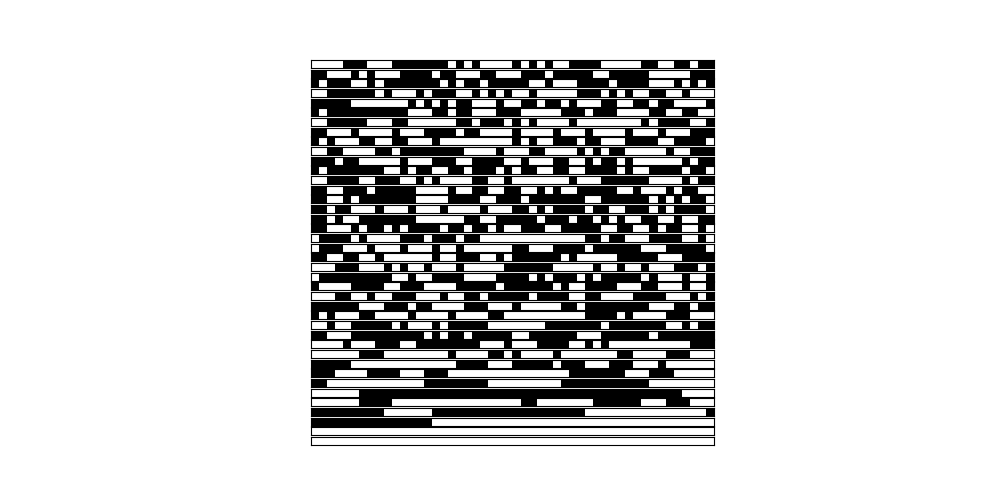
\includegraphics[trim = 20mm 0mm 20mm 0mm, clip, width=\linewidth]{Ising1DPattern}
\caption{1-D Ising chain simulation results}
\label{fig:Ising1DPattern}
\end{figure}

We see that at low temperatures (the lower lines in the diagram), the system settles in a state where all spins are either upwards or downwards oriented. This is clearly the lowest possible value of the energy. For higher temperatures, we see fluctuations aways from this stable point, and some spins point upwards while others point downwards. 

\begin{figure}[ht]
\centering
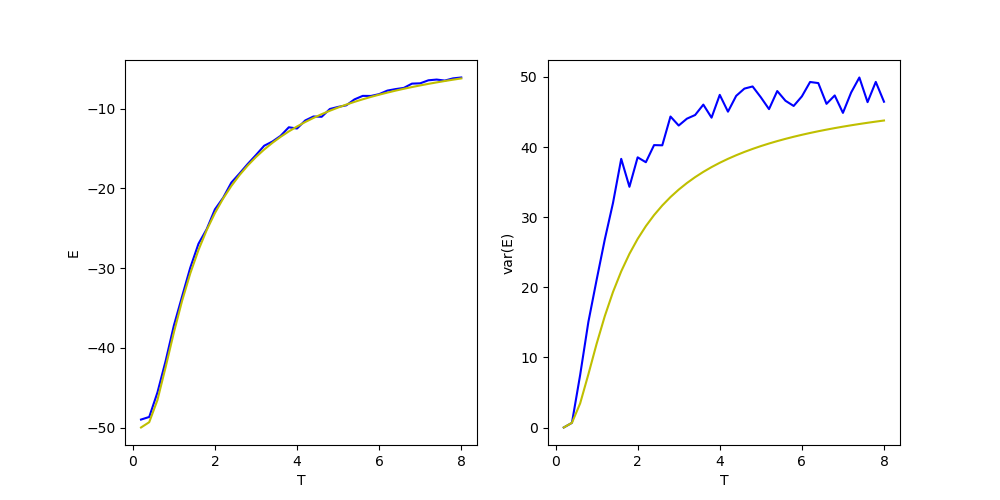
\includegraphics[width=\linewidth]{Ising1DValues}
\caption{1-D Ising model simulation results}
\label{fig:Ising1DValues}
\end{figure}

In diagram \ref{fig:Ising1DValues}, we see the sampled values for the energy and the variance of the energy from the same simulation run. The diagram on the left hand side shows the energy in blue for different temperatures, while the theoretical value has been added in yellow. Both graphs nearly overlap, so the simulation reproduces the theoretical prediction nicely. On the right hand side, we see the variance as simulated in blue and the theoretical value in yellow. The result from the simulation is consistently higher than the theoretical prediction, indicating an additional variance due to the simulation itself, but converges towards the theoretical value for higher temperatures.

The situation is different in two dimensions. Diagram \ref{fig:Ising2DPattern} displays the result of a simulation of a 2-dimensional Ising model with a grid of 40x40 spin locations, using the same algorithm as before. Again, the temperature was slowly decreased from $6.0$ down to $0.2$ in steps of $0.2$. For each temperature, 4 million simulation steps were done, then the resulting grid was captured. The top row represents, from the left to the right, the temperatures $6.0, 5.8, 5.6, 5.4$ and $5.2$. Here we see the expected behaviour - patterns with roughly half of the particles in a spin-up position and half of the particles in a spin-down orientation. 

In the bottom row of the diagram, that corresponds to the temperatures $1.0$, $0.8$, $0.6$, $0.4$ and $0.2$, we also see the expected behavior - all spins are oriented in the same direction. However, starting at temperatures $1.8$, we see that large scale patterns start to emerge. especially for the temperatures $2.$ and $2.4$ (rightmost pictures in the fourth row from the top). For these temperatures, entire connected regions display the same orientation of the spins and thus a non-zero mean magnetization. As the temperature rises, these patterns dissolve again.



\begin{figure}[ht]
\centering
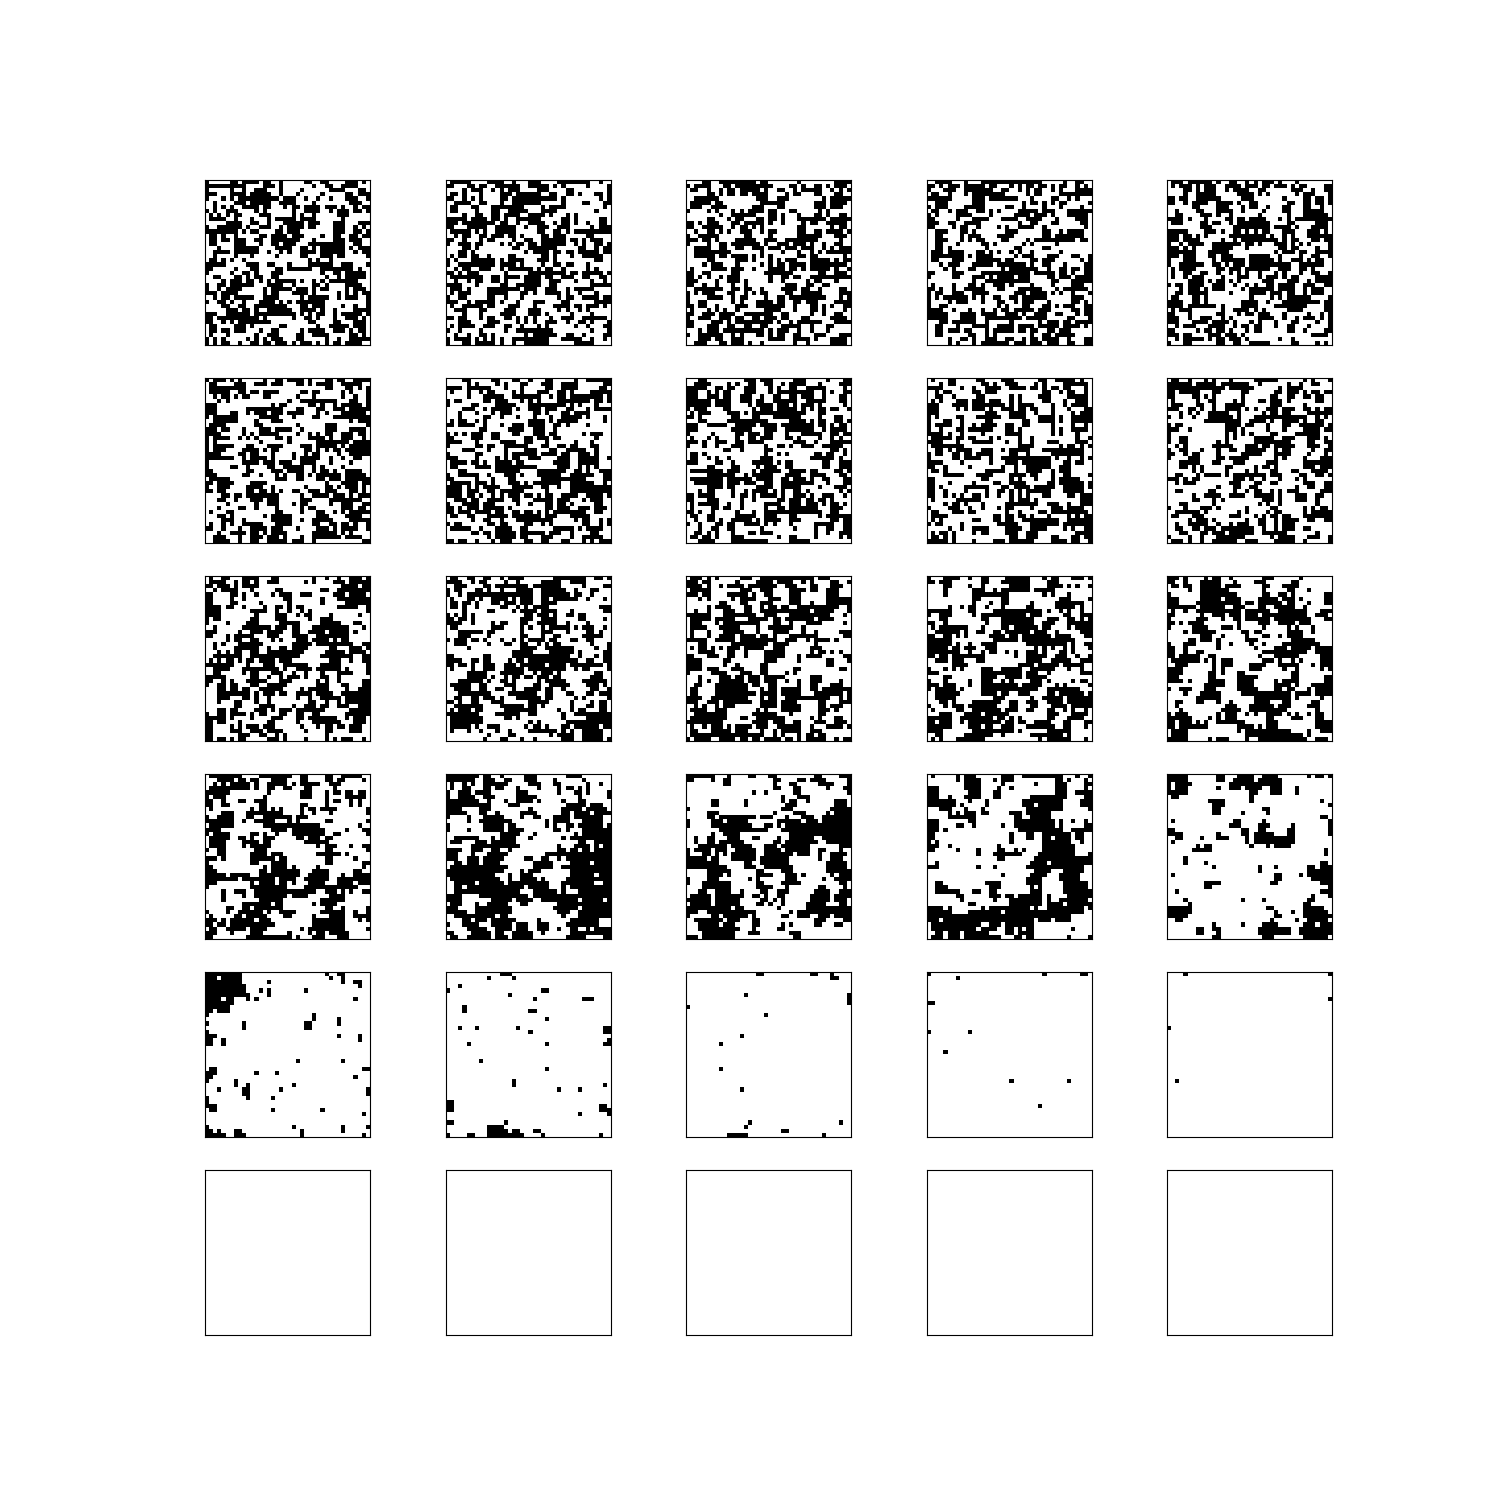
\includegraphics[width=1.0\linewidth]{Ising2DPattern}
\caption{2D Ising model: emerging pattern}
\label{fig:Ising2DPattern}
\end{figure}

The temperature range between $1.8$ and $2.4$ does also display an unusual behavior in plots of mean and variance of the energy, as shown in diagram \ref{fig:Ising2DValues}. 

\begin{figure}[ht]
\centering
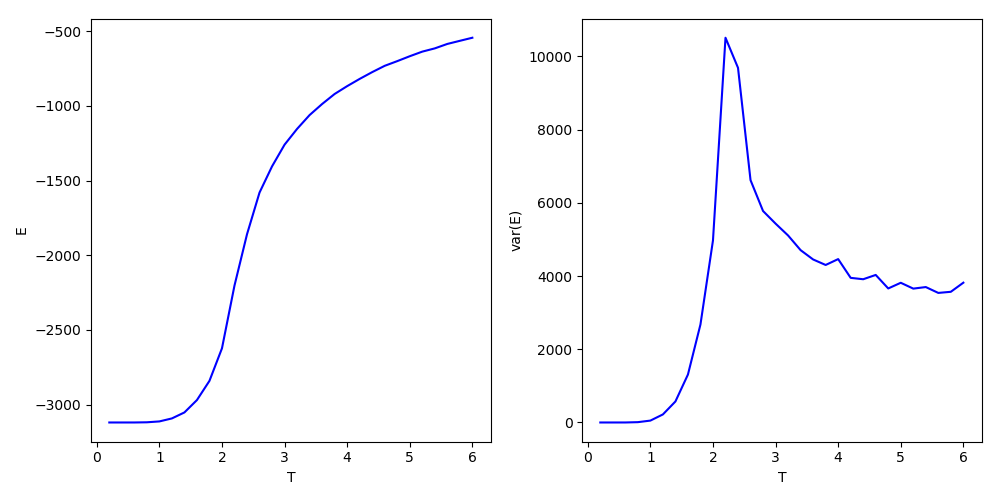
\includegraphics[width=1.0\linewidth]{Ising2DValues}
\caption{2D Ising model: mean and variance of the energy}
\label{fig:Ising2DValues}
\end{figure}

We see that the variance is low for small temperatures, but then rises quickly to  a sharp peak at a temperature of $\approx T = 2.2$ before it decreases again. So in this temperature range, we expect to see strong fluctuations around the state with minimum energy, exactly what we observe in the pattern reproduced above. At this temperature, individual spins combine into larger pattern and long-range correlations evolve, leading to magnetization on a macroscopic scale. This is exactly the type of critical behavior that Ising was looking for and that is absent in one dimension (ironically, Ising, in his own work, came to the wrong conclusion that the model would not exhibit this behavior in any dimension, but of course did not have the power of numerical simulations at his disposal). The temperature where this happens is called the {\em critical temperature} and is predicted to be $T_c \approx 2.27$ by the exact solution of the two-dimensional Ising model in the thermodynamic limit due to Onsager (\cite{Schroeder}), in good accordance with out observations.

It is interesting to print out the average magnetization during such a simulation. Recall that the average magnetization is the sum
$$
M = \sum_i \langle s_i \rangle
$$
Now the Boltzmann distribution is symmetric under the change $s \rightarrow -s$. Therefore the expectation value of any odd function, including all coordinates $\langle s_i \rangle$ and the magnetization is zero. We would therefore assume that when we record the magnetization during a simulation run, we get zero.

Interestingly, for low temperatures, this is not what happens. Instead the system will be attracted by one of the two possible configurations in which all spins are pointing in the same direction, and will be trapped in this local minimum. The reason is that the energy wall between states with almost all spins down and states with almost all spins up is to steep that it is extremely unlikely to cross it during the simulation. Thus, for low temperatures, the Markov chain given by the Gibbs sampler does not really converge, and therefore samples of all functions with odd components will be biased. Put differently, the state space is effectively not connected and the chain will rarely be able to explore both components of the state space.



%%%%%%%%%%%%%%%%%%%%%%%%%%%%%%%%%%%%%%%%%%%%%%
%% Bibliography
%%%%%%%%%%%%%%%%%%%%%%%%%%%%%%%%%%%%%%%%%%%%%%

\begin{thebibliography}{9}
	


\bibitem{RobertCasella1999}
C.P.~Robert, G.~Casella,
{\em Monte Carlo Statistical Methods},
Springer, New York 1999


\bibitem{Schroeder}
D.V.~Schroeder,
{\em An introduction to thermal physics},
Addison-Wesley, San Francisco 2000

\bibitem{MacKay}
D.~MacKay,
{\em Information Theory, Inference and Learning Algorithms},
Cambridge University Press, Cambridge 2003

\bibitem{Ising1924}
E.~Ising,
{\em Beitrag zur Theorie des Ferromagnetismus},
Zeitschrift f. Physik, Vol. 31, No.1 (1924), 253--258

\end{thebibliography}
\end{document}


